\chapter{Metodologia}
\label{cap:metodologia}

\section{Coleta de Dados}
\label{sec:col_dados}
Para esta pesquisa, será utilizada uma amostra de uma base de dados extraídas do \gls{NPM}. Esta base contém informações sobre todos os pacotes hospedados no \gls{NPM} até jun/2017, totalizando \textit{366,629} pacotes. Para cada pacote, há informações sobre cada uma de suas \textit{releases}. A Tabela \ref{tab:database} contém as informações para o pacote \textit{buffer-includes}\footnote{https://npmjs.org/package/buffer-includes}:

\begin{itemize}
    \item \textit{name}: o nome do pacote;
    \item \textit{version}: as versões de cada \textit{release} do pacote;
    \item \textit{timestamp}/\textit{prev\_timestamp}: contêm os \textit{timestamp} relacionados àquela determinada \textit{release};
    \item \textit{prov\_name}: os nomes dos provedores daquela \textit{release};
    \item \textit{prov\_vers}: contém, no momento da \textit{release} do cliente, a última versão dos provedores que o cliente aceitava; e
    \item \textit{prov\_chng}: informa o tipo de atualização que os provedores realizaram desde a última \textit{release} do cliente:
    \begin{itemize}
        \item se vazio: o provedor foi adicionado nesta \textit{release};
        \item \textit{steady}: a versão aceita do provedor não foi alterada desde a última \textit{release} do cliente, ou seja, o provedor não publicou nenhuma \textit{release} aceita pelo cliente; e
        \item \textit{upgrade}: após a última \textit{release} do cliente, o provedor publicou uma nova \textit{release} que o cliente aceita.
    \end{itemize}
\end{itemize}{}
  
\begin{table}[!h]
    \scalebox{0.72}{
        \begin{tabular}{|c|c|c|c|c|c|c|c|}
            \hline
            name & version & timestamp & prev\_timestamp & prov\_name & prov\_vers & prov\_chng \\ \hline
            buffer-includes & 0.1.0 & 2015-10-28T09:14:25.805Z &  & buf-indexof & 1.0.0 &  \\ \hline
            buffer-includes & 0.1.0 & 2015-10-28T09:14:25.805Z &  & ava & 0.3.0 &  \\ \hline
            buffer-includes & 0.1.0 & 2015-10-28T09:14:25.805Z &  & xo & 0.10.0 &  \\ \hline
            buffer-includes & 1.0.0 & 2016-09-30T08:23:30.480Z & 2015-10-28T09:14:25.805Z & buf-indexof & 1.0.0 & steady \\ \hline
            buffer-includes & 1.0.0 & 2016-09-30T08:23:30.480Z & 2015-10-28T09:14:25.805Z & ava & 1.0.0 & upgrade \\ \hline
            buffer-includes & 1.0.0 & 2016-09-30T08:23:30.480Z & 2015-10-28T09:14:25.805Z & xo & 0.16.0 & upgrade \\ \hline
        \end{tabular}
    }
    \caption{Formato da base de dados para cada pacote do NPM}
    \label{tab:database}
\end{table}

A base contém um total de \textit{366K} de projetos e por isso, realizar uma análise manual para um número gigantesco de projetos não é viável. Por isso, será utilizado uma amostra para o estudo de 384 pacotes, com base em um cálculo amostral\footnote{https://pt.surveymonkey.com/mp/sample-size-calculator/} com 95\% de confiança e 5\% de margem de erro. Dos \textit{366K} de pacotes, a amostra de 384 pacotes foi recuperada sorteando um número no intervalo \textit{0-366,629}. Do pacote sorteado, foi recuperado o seu \textit{package.json} e verificado se o pacote cumpre quatro requisitos: possui mais de 1 provedor --  se não houver provedores, não há possibilidades do pacote sofrer \textit{breaking changes}; possui um \textit{script} de teste não vazio e diferente do \textit{script} padrão de teste do \gls{NPM}: \textit{Error: no test specified}; possui a \textit{url} do repositório do pacote; e o repositório do pacote precisa existir -- será esperado de uma requisição \Gls{HTTP} para o repositório o código \textit{200} indicando sua existência. Todos esses requisitos foram analisados recuperando a \textit{release latest} do pacote, ou seja, a última \textit{release} disponível. A Figura \ref{fig:package_json} exemplifica as informações pertinentes no \textit{package.json} do pacote \textit{buffer-includes@1.0.0}\footnote{http://registry.npmjs.org/buffer-includes}.

\begin{figure}
    \centering
    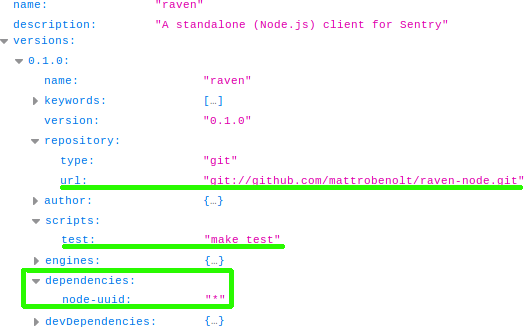
\includegraphics[scale=0.7]{figuras/package_json.png}
    \caption{Informações que serão recuperadas do \textit{package.json} para validar um pacote}
    \label{fig:package_json}
\end{figure}{}

Inicialmente, foram sorteados e executados 384 pacotes para o estudo, mas em 22 destes pacotes não foi possível executar o comando \textit{npm install}/\textit{npm test} para nenhuma de suas \textit{releases}. Isso porque estes pacotes apresentaram algum tipo de erro que impossibilitou a execução. Destes 22 pacotes, 15 não possuíam algum dos arquivos necessários para os testes; 4 haviam listados alguns dos arquivos no \textit{.gitignore}, mas que eram necessários para a execução; 2 necessitaram de configurações específicas em banco de dados mas que não foi possível realizá-las;e 1 pacote foi considerado como um \textit{toy package}, ou seja, não era um projeto real, apenas um repositório no qual o desenvolvedor, provavelmente, criou para testar o \gls{NPM}. Então, os 22 pacotes foram substituídos em um novo sorteio seguindo o mesmo critério, totalizando 384 pacotes com 4570 \textit{releases} que foram utilizados no estudo. A Figura \ref{fig:database} apresenta a distribuição de provedores e de \textit{releases} entre a base e a amostra, na qual os \textit{boxplots} em azul -- dois primeiros -- representam a amostra e os \textit{boxplots} em vermelho -- dois últimos -- representam a base de dados.

\begin{figure}
    \centering
    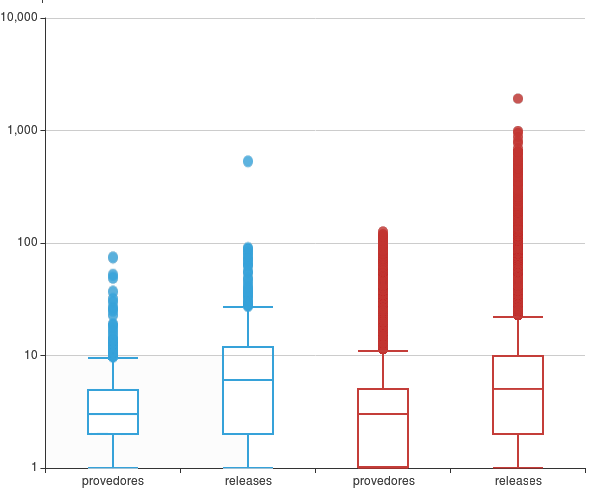
\includegraphics[scale=0.6]{figuras/data_box_plot_pt.png}
    \caption{Distribuição de provedores e \textit{releases} da amostra e da base, respectivamente}
    \label{fig:database}
\end{figure}{}

Em ambos os \textit{boxplots} da Figura \ref{fig:database}, o terceiro quartil e a mediana valem, respectivamente, 5 e 3 para os provedores. A maior discrepância visível nesta Figura é o quartil 1 entre os \textit{boxplots} dos provedores, uma vez que a quantidade de provedores, por pacote, abaixo da mediana representam 44\% para a amostra e 47\% para a base de dados, e esta discrepância aumenta conforme o número de provedores diminui. Já o terceiro quartil e a mediana dos \textit{boxplots} das \textit{releases} valem, respectivamente, 12 e 5 para a amostra e 10 e 5 para a base de dados. Por fim, o primeiro quartil vale 2 para ambos os \textit{boxplots} das \textit{releases}. Desta maneira, a amostra consegue representar suficientemente a base de dados.

Um detalhe importante se refere aos pactes que utilizavam algum tipo de sistemas terceiros de banco de dados como o \textit{MySql\footnote{https://www.mysql.com}, Redis\footnote{https://redis.io}} entre outros sistemas. Então, quando um erro foi ocasionado pela falta de um destes sistemas, fez-se a habilitação e o pacote foi re-executado. Somente quando o pacote necessitava de uma configuração específica e que não foi possível executá-la, então este pacote foi substituído por outro.

\section{Ferramenta \textit{BCDetect} para executar os pacotes}
\label{sec:bcdetect}
Para executar os pacotes, foi desenvolvida uma ferramenta chamada \textit{BCDetect} disponível no \textit{GitHub}\footnote{https://github.com/danielventurini/bcdetect} sob a licença \textit{MIT}\footnote{https://choosealicense.com/licenses/mit}. Esta ferramenta recebe um arquivo de entrada no padrão da Tabela \ref{tab:database} e clona o repositório do respectivo pacote -- coincidentemente, todos os repositórios dos pacotes sorteados estavam hospedados no \textit{GitHub}. Após, é criado uma estrutura de dados para armazenar as informações extraídas do arquivo de entrada, na qual cada \textit{release} contém todas os provedores com suas versões e o tipo de atualização que os provedores realizaram desde a última \textit{release} do cliente. Esta estrutura está representada na Figura \ref{fig:bc_work}, que seria construída a partir da Tabela \ref{tab:database}.

\begin{figure}
    \centering
    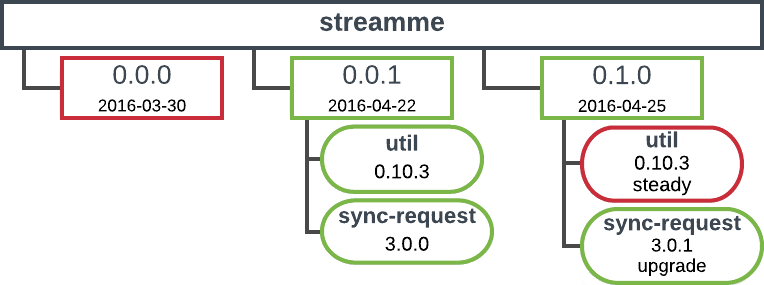
\includegraphics[scale=2]{figuras/bcdetect_work.png}
    \caption{Estrutura de dados para representar o arquivo de entrada da Tabela \ref{tab:database}}
    \label{fig:bc_work}
\end{figure}{}

Se uma \textit{release} houver provedores adicionados ou com novas versões aceitas -- \textit{upgrade} --, é executado o comando \textit{git checkout} para restaurar a \textit{working tree} -- arquivos e sub-diretórios do repositório -- para a data da \textit{release} do cliente. Ao alterar a \textit{working tree}, todos os arquivos são restaurados para exatamente os mesmos arquivos do momento em que o cliente publicou a \textit{release}. Então o arquivo \textit{package-lock.json}\footnote{https://docs.npmjs.com/files/package-lock.json} é excluído -- se houver --, pois este arquivo altera o comportamento do comando \textit{npm install} -- a partir do \textit{NPM@5} -- fazendo com que o \gls{NPM} instale as versões dos provedores de acordo com o \textit{package-lock.json}, e não de acordo com o \textit{package.json}. Após, é atualizado a versão dos provedores no campo \textit{dependencies} do \textit{package.json} para suas versões que foram recuperadas do arquivo. Esta operação não diferencia os provedores que estão no \textit{dependencies} ou no \textit{devDependencies}\footnote{além, há outros campos para dependências no \textit{package.json}, tais como o \textit{peerDependencies}, \textit{optionalDependencies} e o \textit{globalDependencies}}, uma vez que, para realizar o \textit{test}, ambos os provedores são requeridos. Por fim, é alterado a versão do \textit{Node.js} para a versão contida no campo \textit{engines\textrightarrow node} -- se houver -- no \textit{package.json} ou para a mais recente utilizando como referência a data da \textit{release} do cliente.

Para realizar a alteração da versão do \textit{Node.js} é utilizado como referência a data da \textit{release} do cliente. Através desta data, é possível identificar a última \textit{release} do \textit{Node.js} disponível\footnote{https://nodejs.org/en/download/releases} no momento da \textit{release} do cliente, ou seja, qual é a \textit{release} máxima do \textit{Node.js} que o cliente executou o pacote. Assim, o pacote é executado em todas as versões \textit{major} do \textit{Node.js}, da versão mais atual, pela data da \textit{release} do cliente, até a versão \textit{major} mais antiga. Para o pacote da Tabela \ref{tab:database}, a sua \textit{release 0.1.0} possui o \textit{timestamp 2016-04-25}, e a última \textit{release} do \textit{Node.js} disponível até esta data é a \textit{4.4.3}. Assim, este pacote foi executado com uma \textit{release 4.x, 3.x, 2.x, 1.x, 0.x} do \textit{Node.js}, até que uma dessas resultassem em sucesso na execução. Este chaveamento de versões do \textit{Node.js} é necessário pois um pacote que executa com sucesso na versão \textit{0.x} do \textit{Node.js}, por exemplo, provavelmente não irá executar com sucesso na versão \textit{8.x} do \textit{Node.js}. Desta forma, toda vez que a execução do pacote resulta em erro, é alterado a versão do \textit{Node.js} para a próxima \textit{release major} inferior e novamente é executado o pacote. Analogamente, esse problema de versões atinge o \gls{NPM}, mas ao alterar a versão do \textit{Node.js}, a versão do \gls{NPM} é atualizado também. Por fim, o \textit{BCDetect} salva as seguintes informações:

\begin{itemize}
    \item versão do pacote cliente;
    \item se houve alteração na versão aceita de alguns dos provedores;
    \item os códigos da execução do \textit{npm install} e \textit{npm test} -- sucesso ou erro;
    \item a versão do \textit{Node.js} que deveria ser executado com base na data da \textit{release}; e
    \item a versão do \textit{Node.js} que realmente o pacote executou com sucesso.
\end{itemize}{}